%% ID: metal_bar
%% TITLE: Metal bar see-saw
%% TYPE: question
%% QUESTIONTYPE:  numerical
%% CONCEPTS: forces, moments, newtoni
%% VIDEOS: 
%% LEVEL: 3
%% TOPIC: mechanics/statics
%% ORDER: 6

\begin{problem}[IntA1987PSIIQ3l] %moments
{\exposition{A long uniform metal bar of mass \valuedef{M}{1}{kg} is pivoted about its mid-point and three masses are hung from it, the first is a distance \vari{x_1} to the left of the pivot and has a mass \valuedef{m_1}{5}{kg}. The second is a distance \valuedef{x_2}{10}{cm} to the left of the pivot and has a mass \valuedef{m_2}{20}{kg}. The third mass is a distance \valuedef{x_3}{45}{cm} to the right of the pivot and has a mass \valuedef{m_3}{10}{kg}. The whole system is in equilibrium.}

\nl \question{Calculate the reaction force at the pivot and find the distance \vari{x_1}.}}
{\textit{Used with permission from UCLES, A Level Physical Science, November 1987, Paper 2, Question 3}}
{\answer{\valuedef{R}{352.8}{N;} \valuedef{x_1}{0.5}{m}}
Figure \ref{fig:Statics_balancing} shows the forces on the bar:
\begin{figure}[h]
\centering
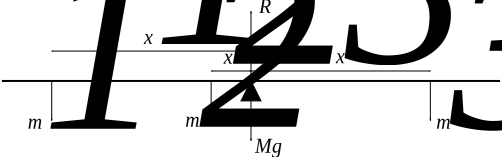
\includegraphics[width=11cm]{Statics_balancing}
\caption{}
\label{fig:Statics_balancing}
\end{figure}
\\
To find \vari{R} all we need to do is resolve forces vertically, to find
\begin{align*}
R=m_1g+m_2g+m_3g+Mg=352.8\textrm{ N}
\end{align*}
To find \vari{x_1}, we can just take moments about any point (other than \vari{x_1} itself). About the centre we have:
\begin{align*}
m_1x_1+m_2x_2&=m_3x_3 \\
\Rightarrow x_1&=\frac{m_3x_3-m_2x_2}{m_1}=0.5\textrm{ m}
\end{align*}
}
\end{problem}